\chapter{Preliminary  Design}

\section{Tools of data flow strategy}
	% Data flow strategy shows th and their interactions...........\\
	Data flow strategy shows the use of data in the system pictorially. The tools
	use in following this strategy show all the essential features of the system and
	how they fit together. It can be difficult to fully understand a business process
	through a verbal description alone; data flow tools help by illustrating the
	essential components of a system and their interactions.\\
\textbf{Data flow analysis makes use of the following tools:}\\
% Flow Charts\\
% Data Flow Diagrams\\
% Data Dictionary\\
% \textbf{Flowchart}\\
% Flowchart is used to represent the algorithm .......\\
% \textbf{Data Dictionary}\\
% The logical characteristics of current systems data stores, including name, description, aliases, contents, ..........\\
% \textbf{Data Structure Diagrams}\\
% A pictorial description of the relation between entities (people, places, events and things) in system and the set of information about the entity, .........\\
% \textbf{Structured Chart}\\
% A design tool that pictorially shows the relation between processing modules in computer software, describes .............

\begin{itemize}
    \item \textbf{Use Case Diagram}:\\
    Illustrates the interactions between users (actors) and the system, showcasing the functional requirements and major processes.

    \item \textbf{Data Flow Diagrams (DFD)}:\\
    Represent the flow of data within the system. DFDs help visualize how information moves between processes, data stores, and external entities.

    \item \textbf{Entity Relationship Diagram (ER-Diagram)}:\\
    Displays the logical structure of the database, showing entities, attributes, and the relationships among them. It is crucial for designing a consistent and efficient database schema.
\end{itemize}
%-----------------------------------------------------------------

\section{Use Case Diagram}
%If you add information about use case diagram\\
\subsubsection{Usecase Diagram For Admin}
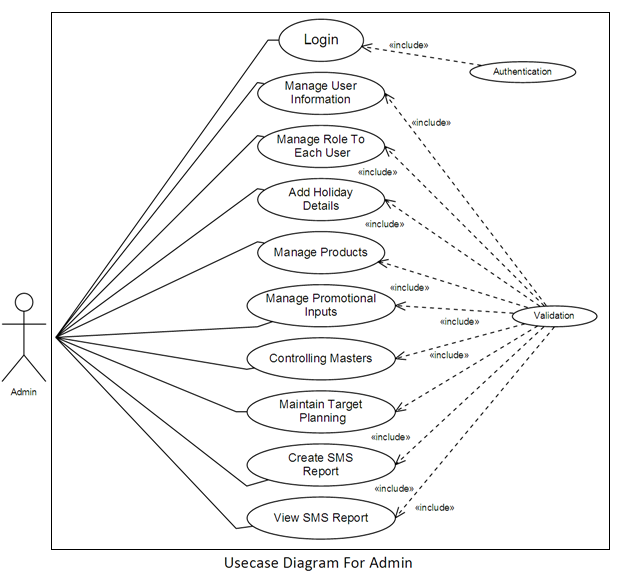
\includegraphics[scale=0.7]{Diag/usecaseadmin.png}

\label{fig:Use case diagram For Admin}
\subsubsection{Usecase Diagram For Other Users.}
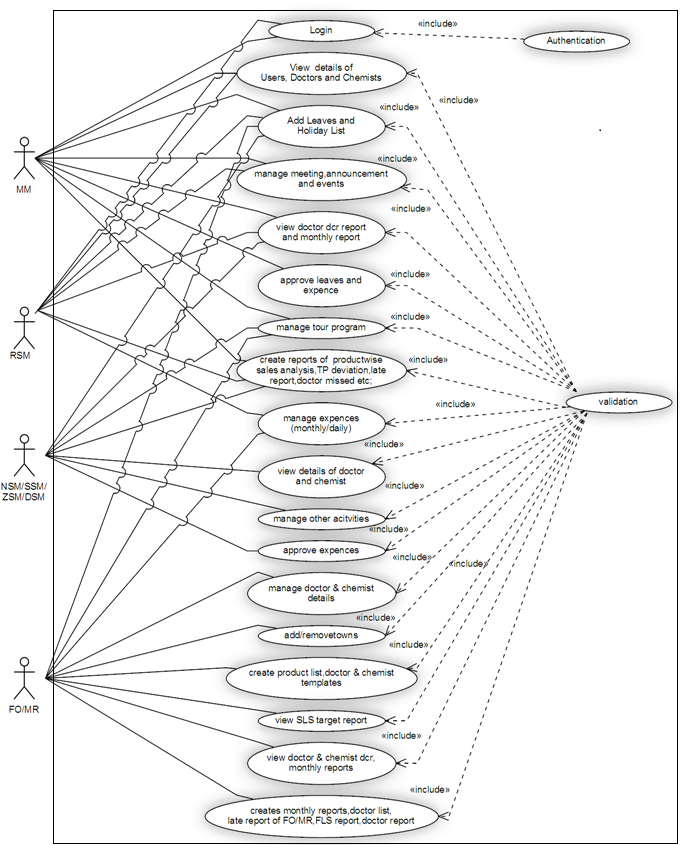
\includegraphics[scale=0.8]{Diag/usecaseall.png}

\label{fig:Use case diagram For Other User}



%-----------------------------------------------------------------
%\section{Activity Diagram}
%%If you add information about Activity Diagram\\
%
%\includegraphics[scale=.8]{Diag/activitylogin.png}
%\label{fig:Activity Diagram}



%-----------------------------------------------------------------

\section{Entity Relationship Diagram}

\subsubsection{ERD For Chemist.}
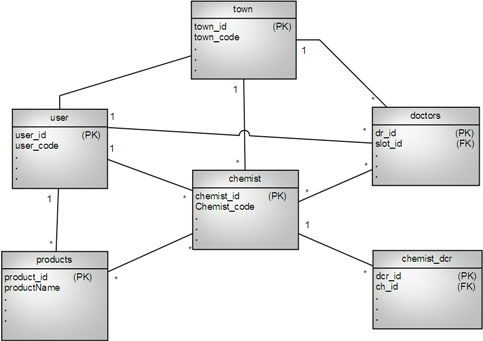
\includegraphics[scale=0.7]{Diag/ERDchemist.png}
\label{abc}

\subsubsection{ERD For doctor.}
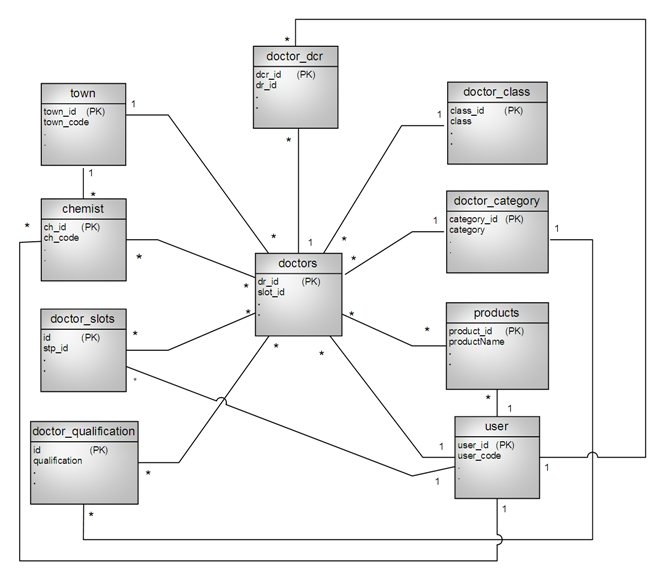
\includegraphics[scale=0.7]{Diag/ERDdoctor.png}
\label{abc}


%\subsubsection{ERD For users.}
%\includegraphics[scale=0.7]{Diag/ERDuser.png}
%\label{abc}
%
%\subsubsection{ERD For Products.}
%\includegraphics[scale=0.7]{Diag/ERDprod.png}
%\label{abc}
%-----------------------------------------------------------------

\section{Data Flow Diagram}
%If you add information about Data flow diagram\\

%\begin{figure} [h]
%\begin{center} 
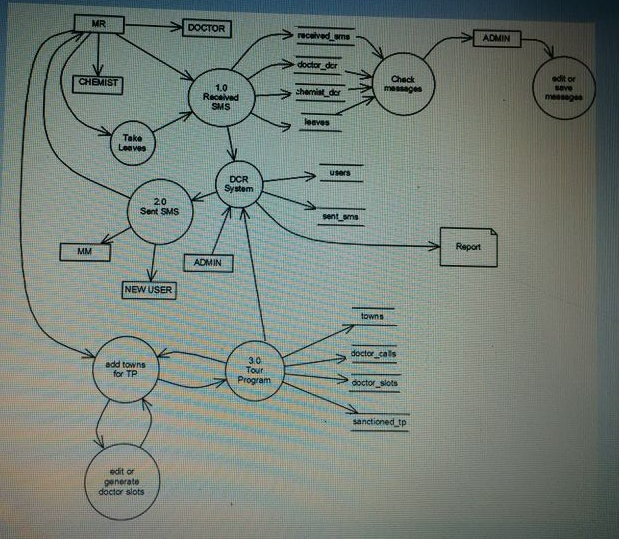
\includegraphics[scale=.9]{Diag/d1.png}
\label{fig:Contex Level}
%\end{center}
%\end{figure}



%\begin{figure} [h]
%\begin{center} 
%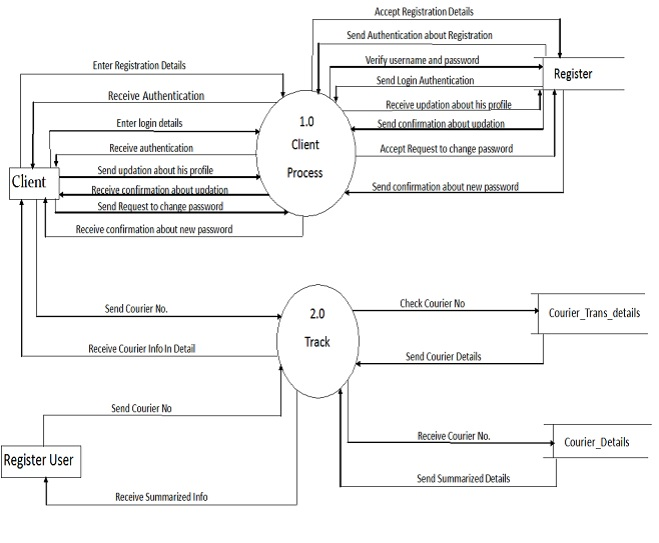
\includegraphics[scale=.9]{Ch5/dfd2.jpg}
%Fig. Data Flow Diagram
%\label{fig:DFD2}


\